\chapter*{Conclusione}

Il fine ultimo del lavoro di tesi era quello di riuscire a realizzare dei modelli di 
workflow per comprenderne la struttura e come possono essere rilevati gli stati 
d’animo, o mood, attraverso delle immagini del volto. 

Ci si era preposti di effettuare questa 
analisi attraverso il framework WoMan che però non ha raggiunto l’obbiettivo 
prefissato in quanto, come è risultato evidente dall’analisi effettuata, vi era necessità di 
diversi altri punti dati per effettuare questo. 

Ho proposto diverse soluzioni per 
risolvere questo problema: la prima è quella di cambiare il dataset utilizzato o di 
modificare quello già presente in modo da risultare maggiormente congiunto allo 
scopo che si voleva raggiungere; la seconda soluzione proposta è quella di fornire 
altri dati al sistema in modo che possa raggiungere i risultati sperati. 

Non ho 
intrapreso nessuna delle due strade in quanto, la prima sarebbe stata troppo dispendiosa in termini di tempo e non sono qualificato alla modifica dei video presenti, mentre, per quanto riguarda la seconda: l’estrapolazione dei dati per i 200 video utilizzati 
è risultata molto dispendiosa di tempo e di energia elettrica, ho optato quindi per mantenere il 
numero di sample a 50 per ognuno dei mood utilizzati. 

Ho però calcolato, attraverso 
la regressione lineare, quanti altri seample servirebbero, vagamente, per arrivare al 
risultato sperato e riporto i risultati ottenuti nelle figure \ref{fig:image36} \ref{fig:image37} \ref{fig:image38} \ref{fig:image39} \ref{fig:image40} 
\begin{figure}
    \begin{center}    
        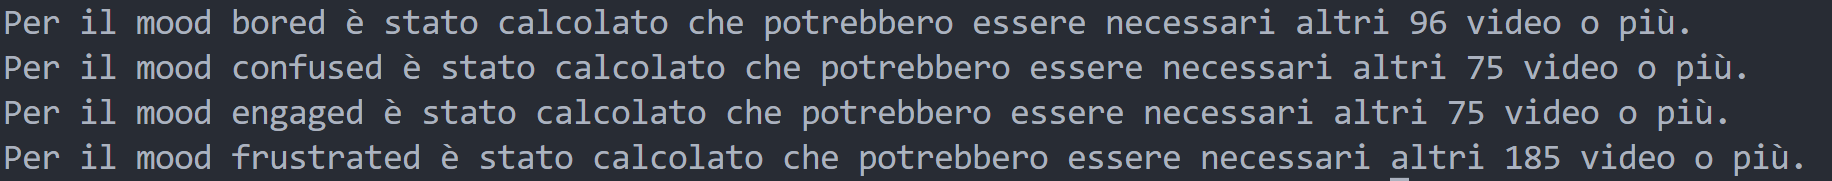
\includegraphics[width=1\linewidth]{images/passaggi aggiuntivi.png}
        \caption{Numero di video aggiuntivi necessari per ogni mood}
        \label{fig:image36}
    \end{center}
\end{figure}
\begin{figure}
    \begin{center}    
        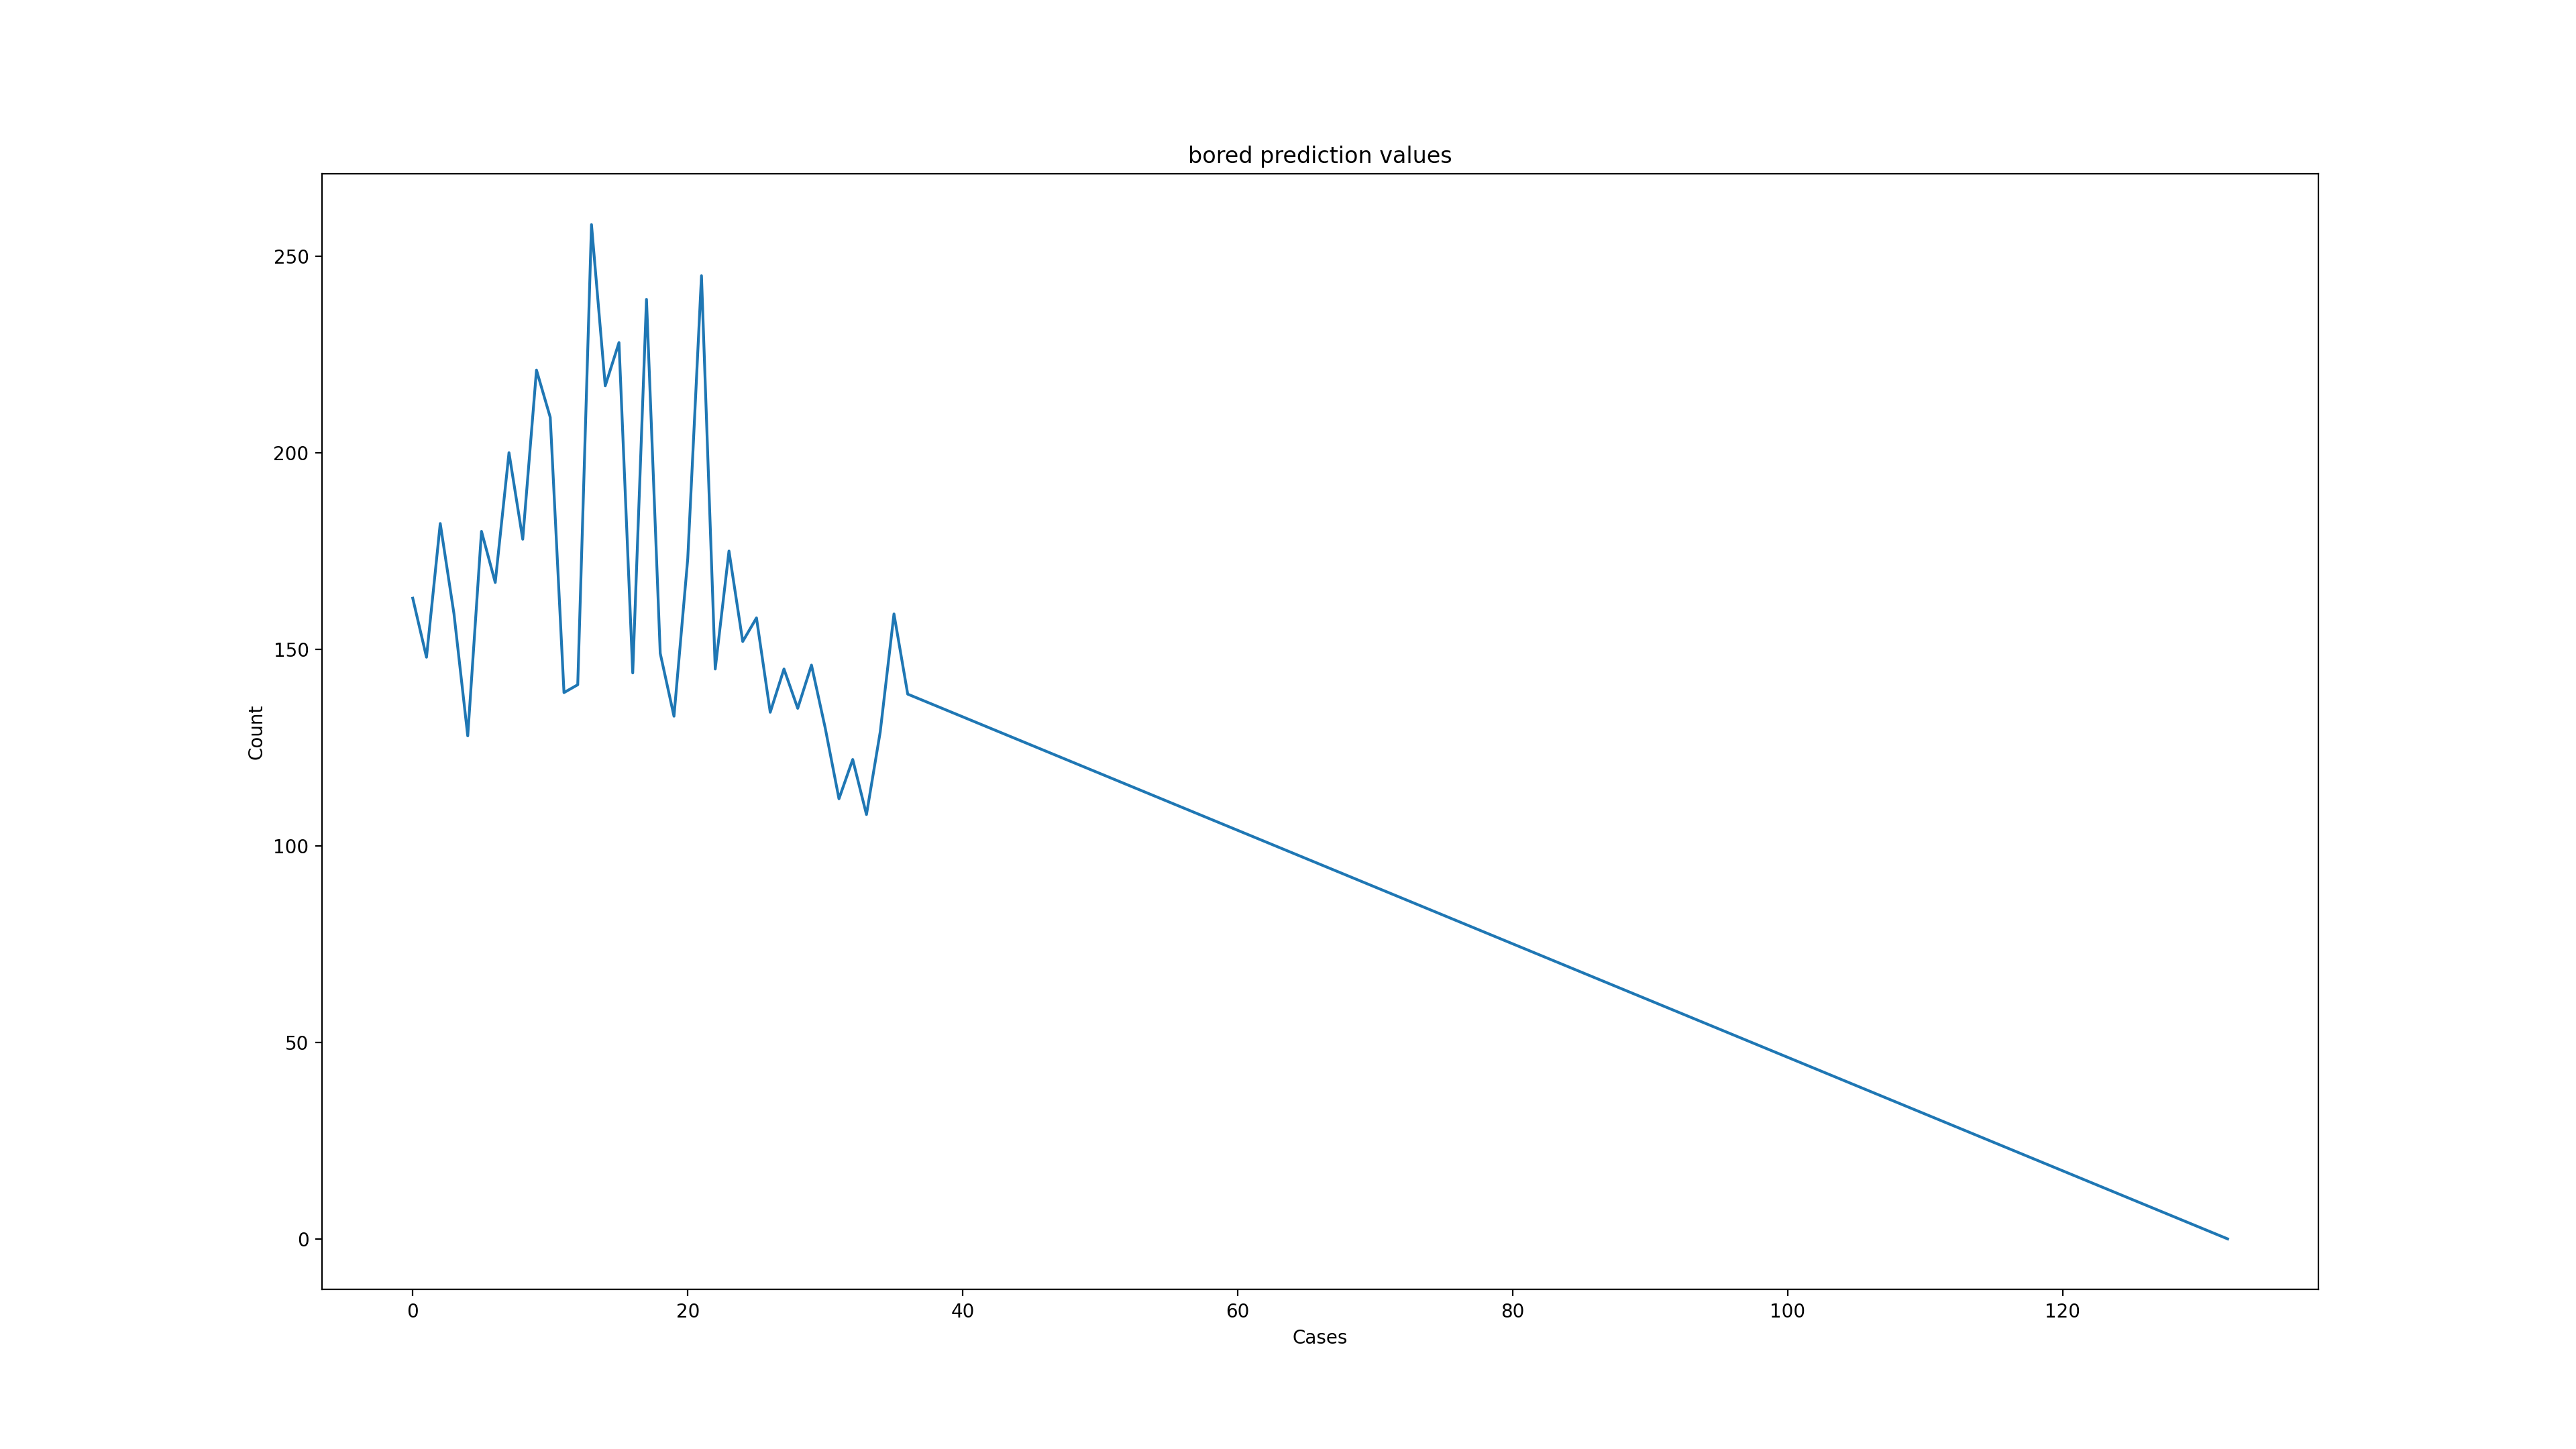
\includegraphics[width=1\linewidth]{images/bored prediction values.png}
        \caption{Valori predetti per il mood Bored}
        \label{fig:image37}
    \end{center}
\end{figure}
\begin{figure}
    \begin{center}    
        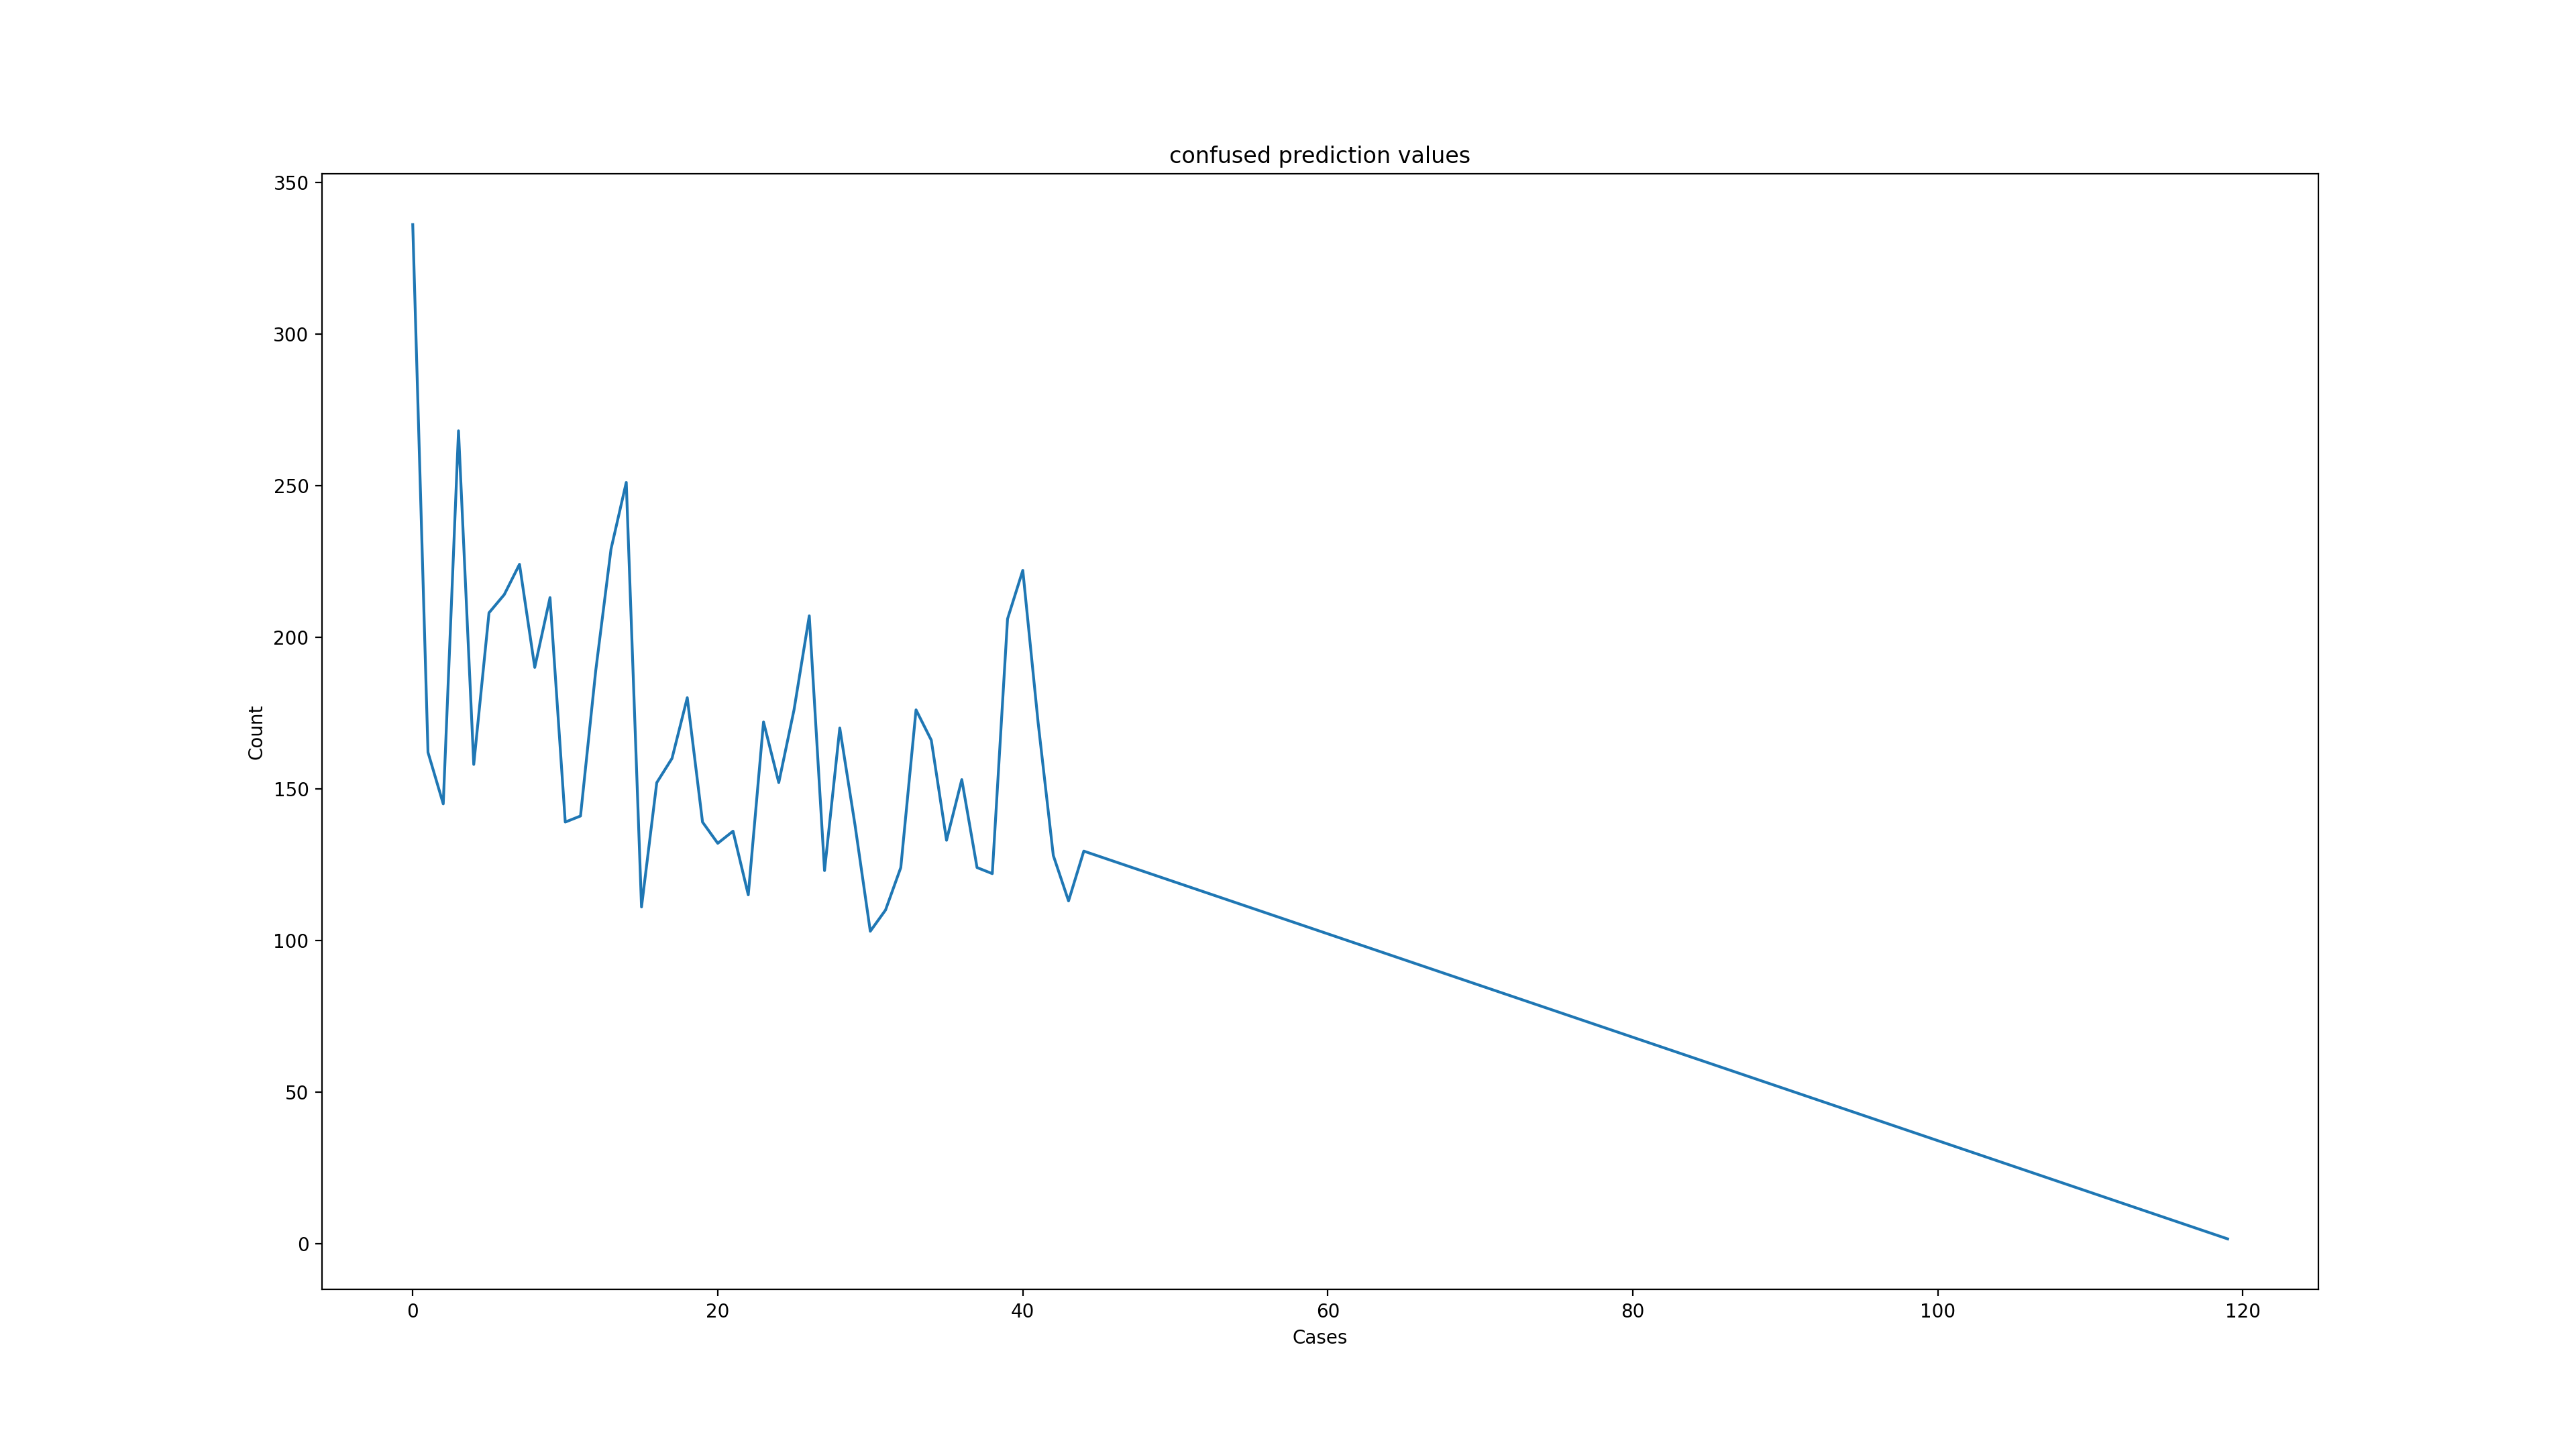
\includegraphics[width=1\linewidth]{images/confused prediction values.png}
        \caption{Valori predetti per il mood Confused}
        \label{fig:image38}
    \end{center}
\end{figure}\clearpage
\begin{figure}
    \begin{center}    
        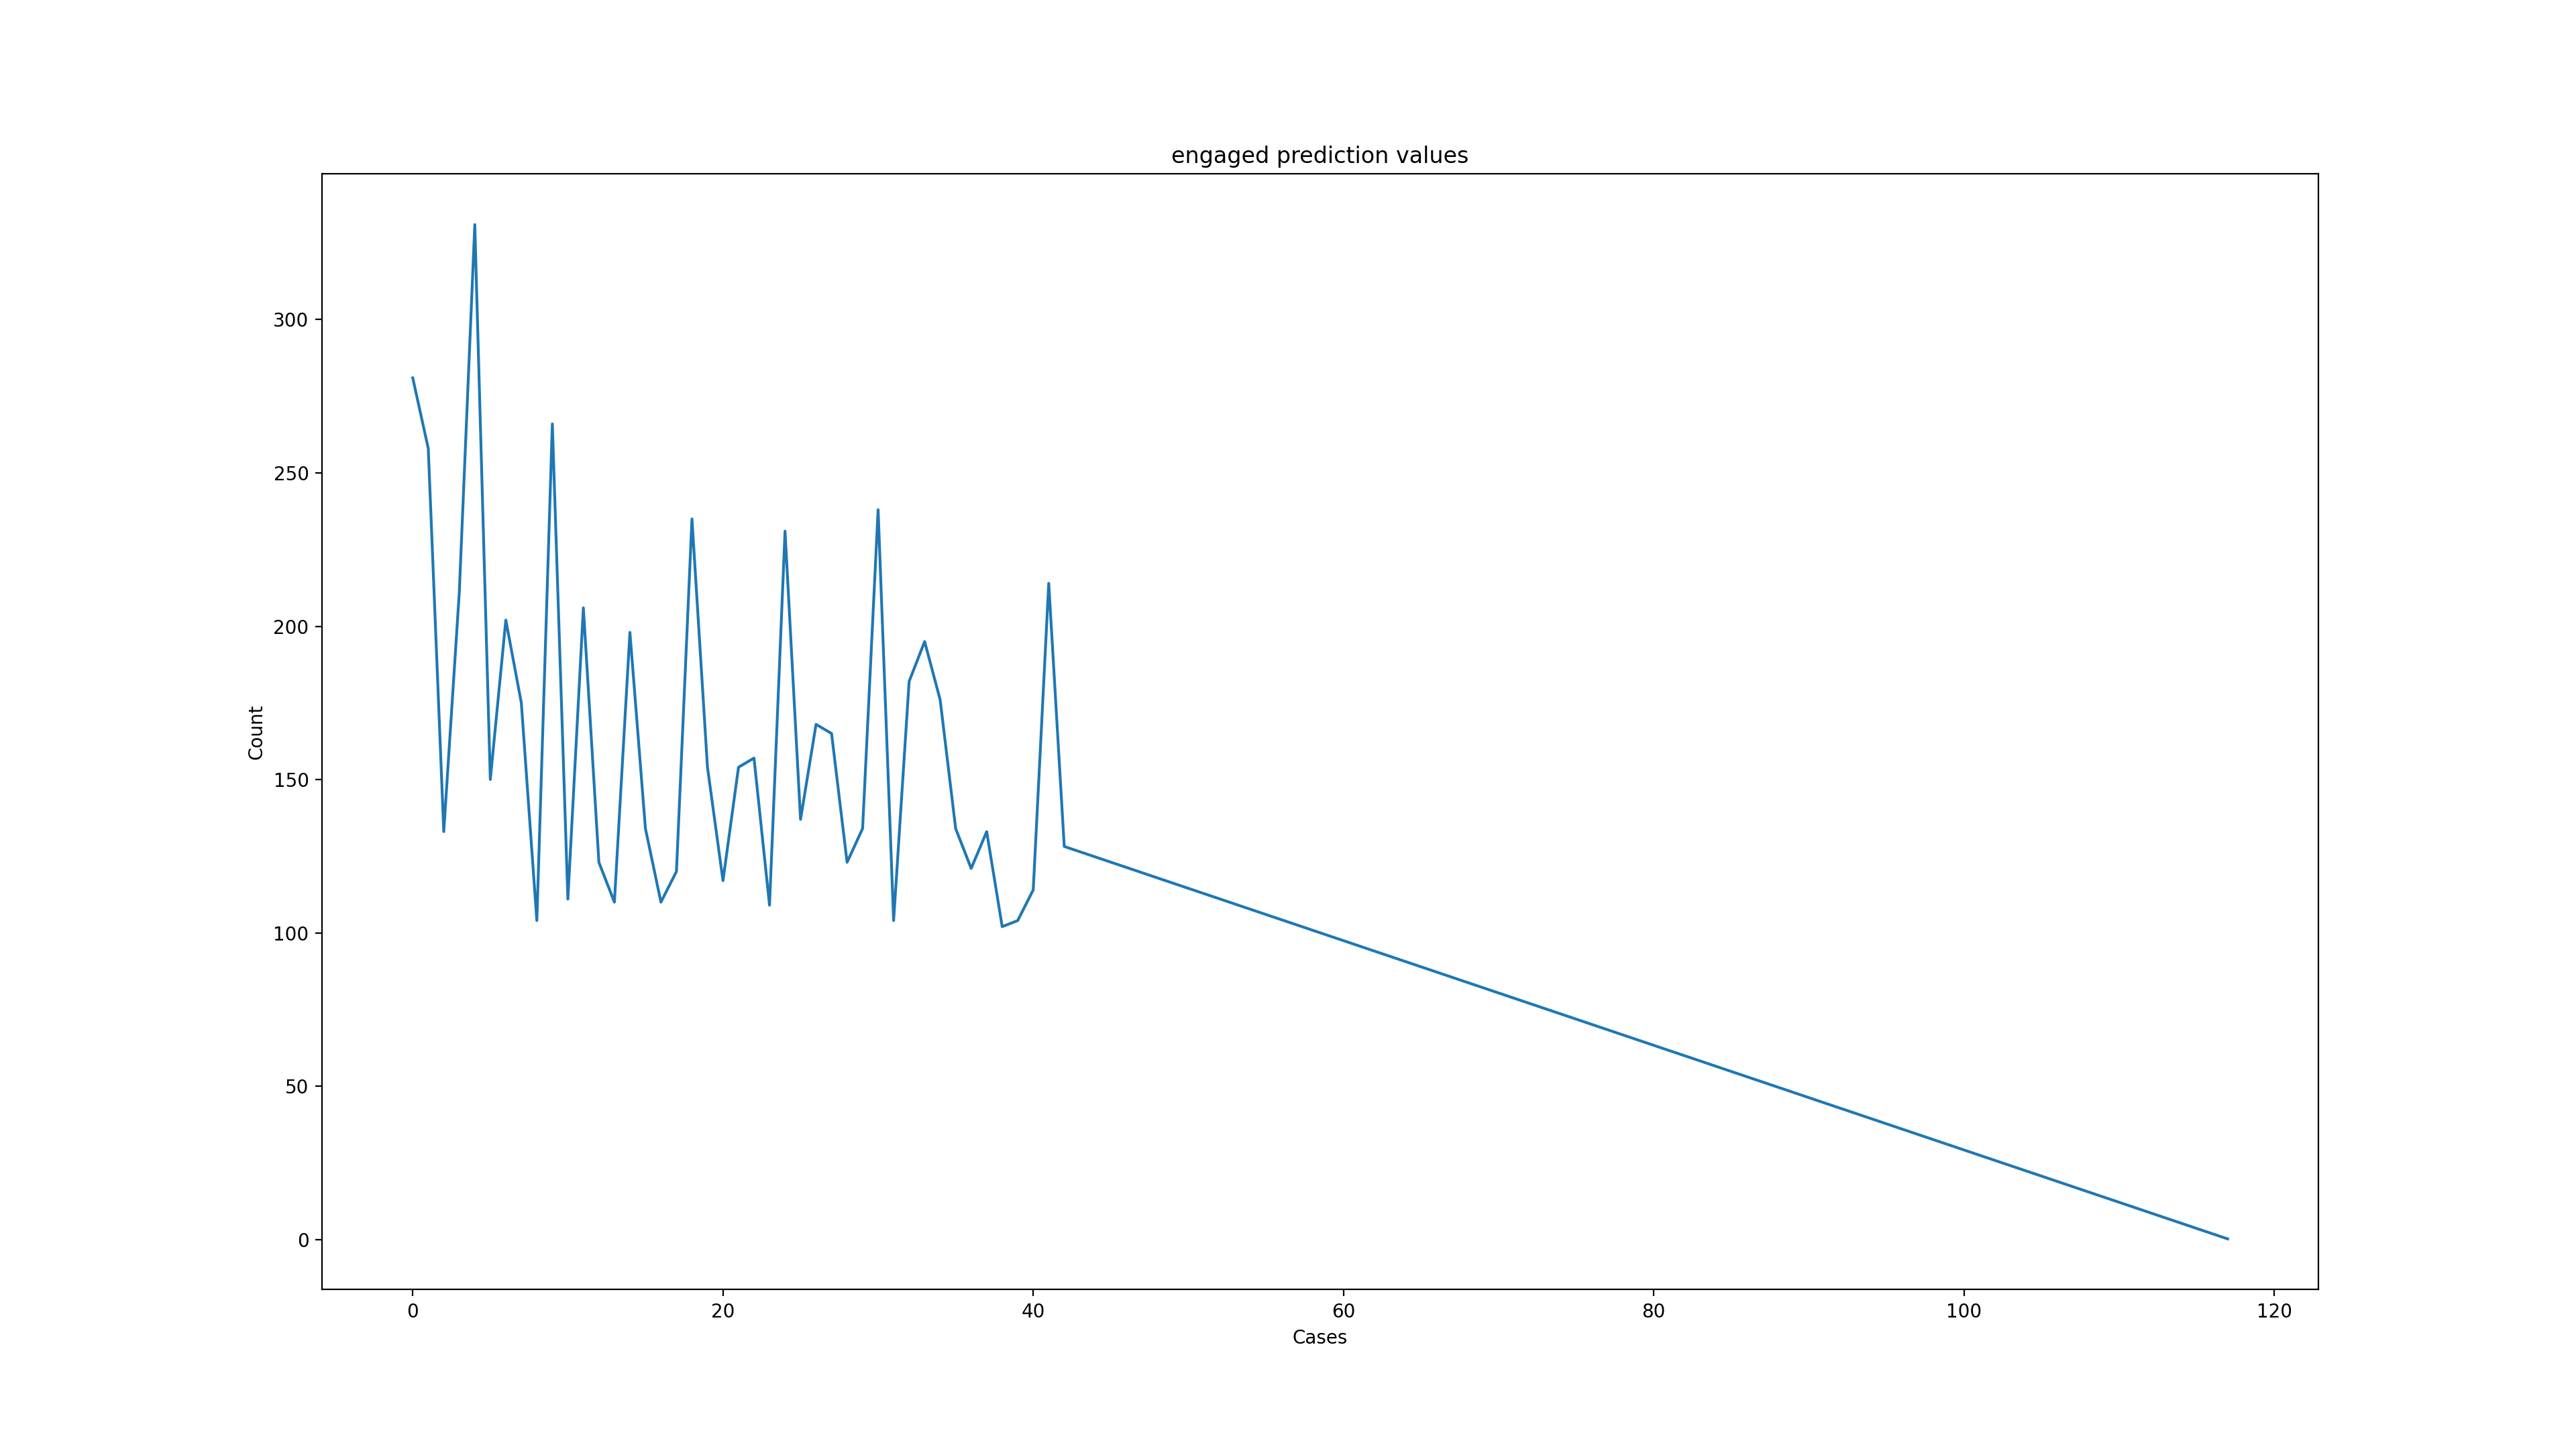
\includegraphics[width=1\linewidth]{images/engaged prediction values.png}
        \caption{Valori predetti per il mood Engaged}
        \label{fig:image39}
    \end{center}
\end{figure}
\begin{figure}
    \begin{center}    
        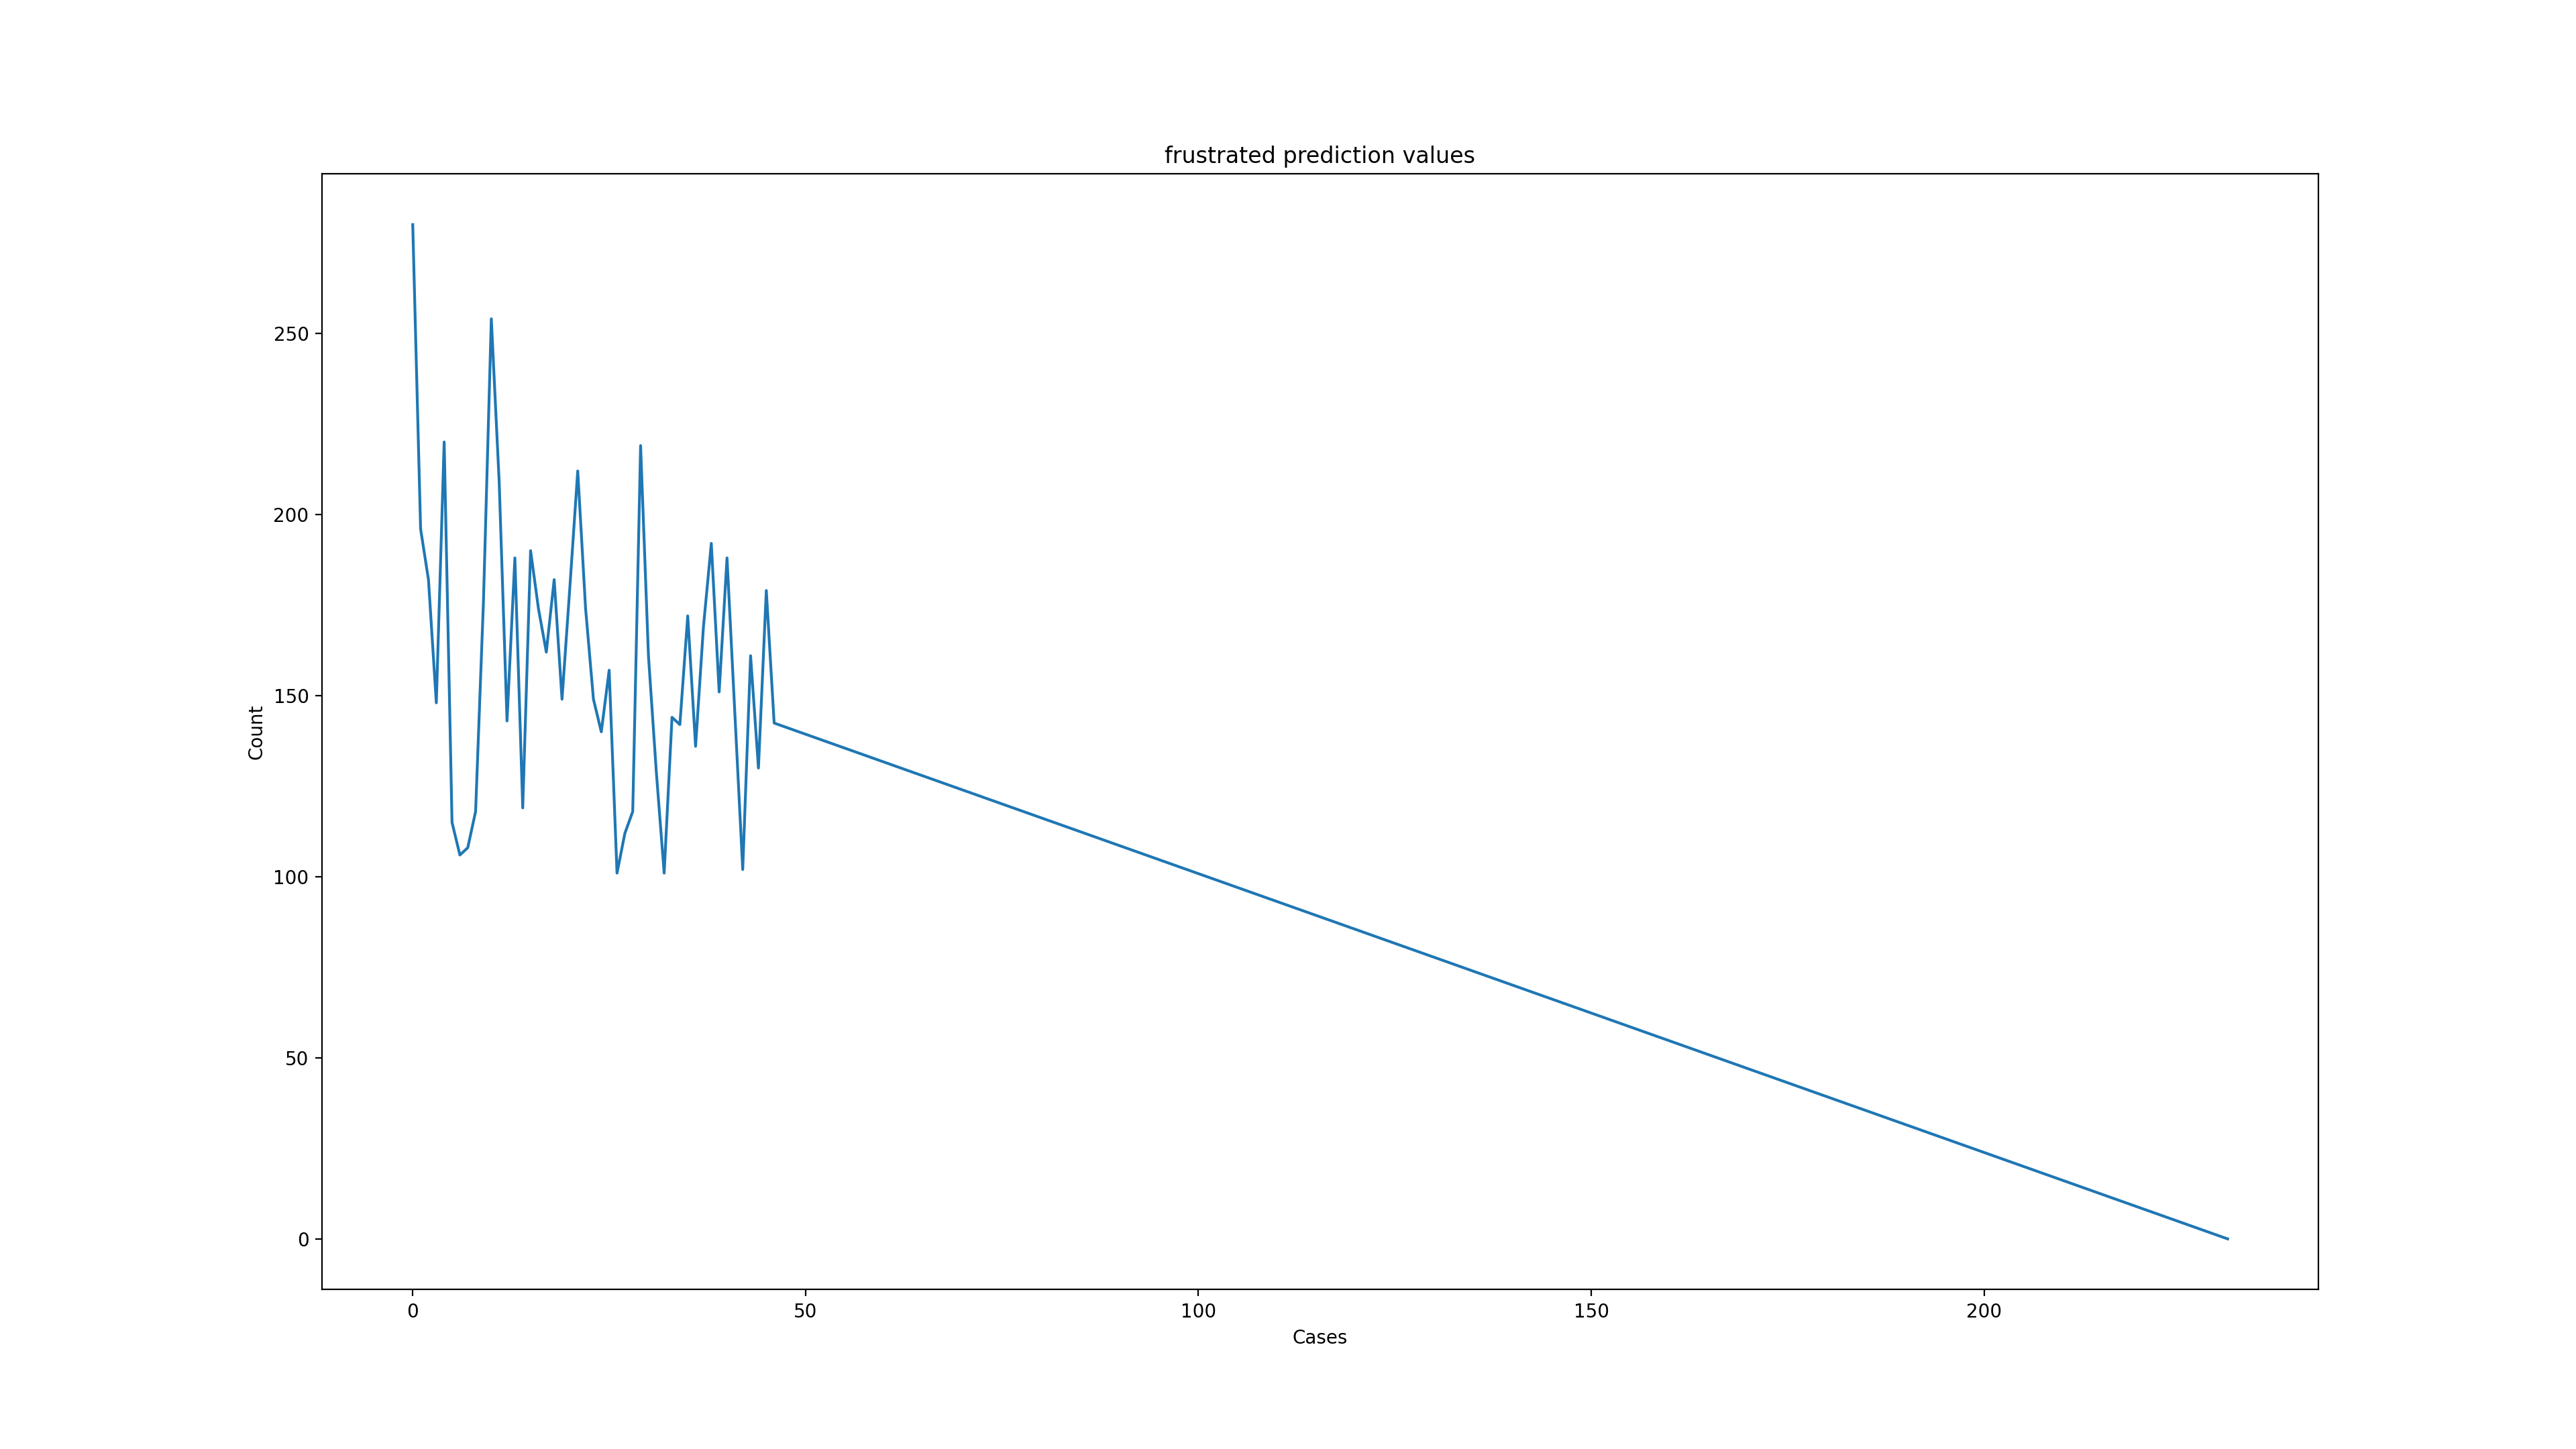
\includegraphics[width=1\linewidth]{images/frustrated prediction values.png}
        \caption{Valori predetti per il mood Frustrated}
        \label{fig:image40}
    \end{center}
\end{figure}

\newpage
In aggiunta a questo studio, come proposto dalla professoressa De Carolis, si è 
presa una strada diversa per la rilevazione dei mood attraverso le espressioni facciali. 

Ho quindi analizzato i diversi studi presenti per l’analisi delle emozioni FACS per poi 
procedere all’applicazione di questi metodi allo studio dei mood. 

Questa strada 
ha portato a risultati migliori ed è anche stato possibile realizzare un applicativo per effettuare delle predizioni in tempo reale utilizzando i modelli predittivi creati (vedi \ref{fig:image35}). 

Difatti, due dei modelli creati sono capaci di effettuare 
delle predizioni con una accuracy intorno all’80\%, nello specifico il Random Forest 
classifier e il KNN classifier (vedi \ref{tab:7}).
\begin{table}
    \small % or \footnotesize
    \caption{Tabella media risultati metriche}
    \label{tab:7}
    \begin{tabular}{ |c||c|c|c|c| } 
         \hline
          & Accuracy & Precision & Recall & Balanced Accuracy\\ 
         \hline\hline
         K-Nearest Neighbors& 77.87493\% & 76.43947\% & 77.87493\% & 77.87465\%\\
         \hline
         Random forest & 82.25838\% & 81.86107\% & 82.25838\% & 82.25838\%\\
         \hline
         Naive bayes& 39.16669\% & 35.96379\% & 39.16669\% & 39.16736\%\\
         \hline
         Support vector machine& 54.37561\% & 53.82087\% & 54.37561\% & 54.38249\%\\
         \hline
         Support vector regressor& 16.62504\% & 18.92075\% & 16.62504\% & 16.6416\%\\
         \hline
    \end{tabular}
\end{table}
\begin{figure}
    \begin{center}    
        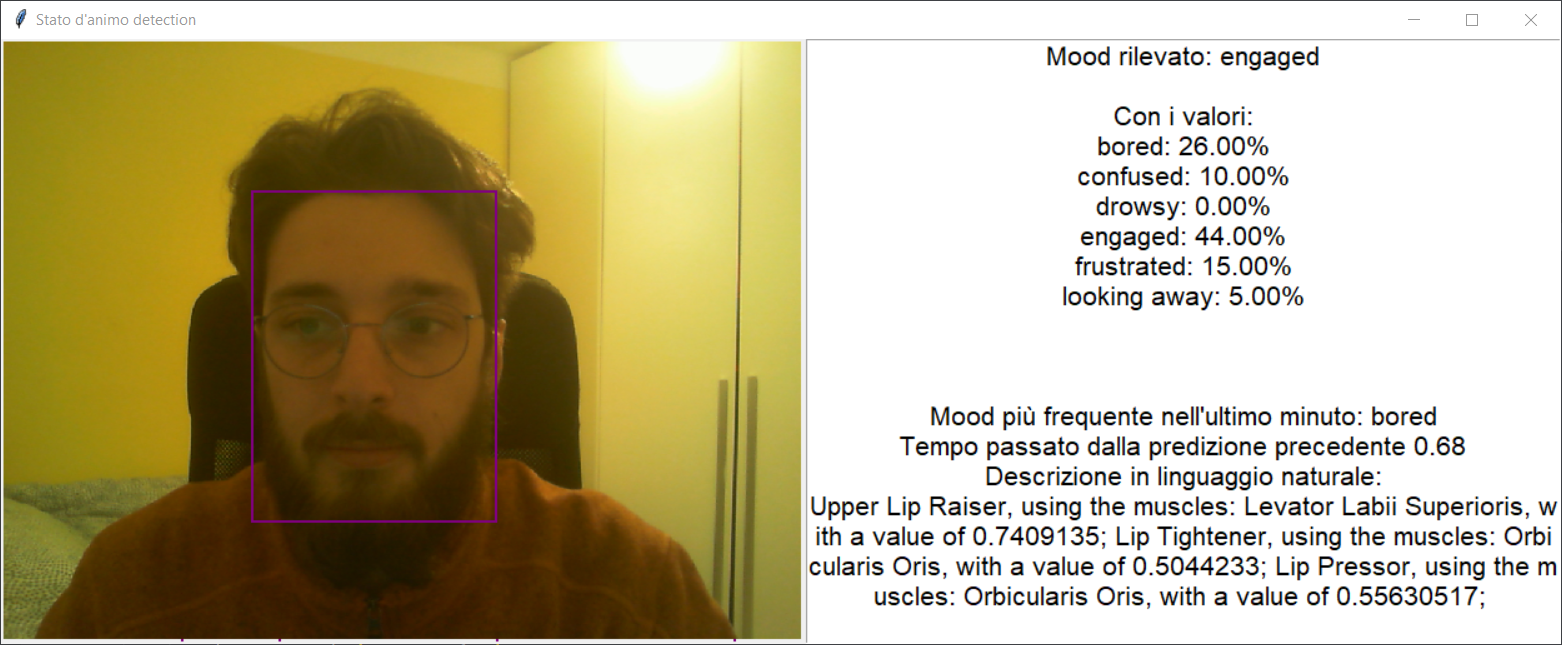
\includegraphics[width=0.9\linewidth]{images/image52.png}
        \caption{Interfaccia per la rilevazione dei mood realizzata}
        \label{fig:image35}
    \end{center}
\end{figure}
